\chapter{Editor umožňujúci konkurentné úpravy jedného dokumentu}

\label{kap:zdialtelnost} % id kapitoly pre prikaz ref

Myšlienka kolaboratývneho editora bola prvýkrát zaznamenaná už v roku 1968 Douglasom Engelbartom. 
Avšak do popularity sa dostala až nedávno, približne 20 rokov od prvého záznamu.
Kolaboratívny editor umožnuje viacerým používateľom upravovať jeden dokument.
Tieto editory sa rozdeľujú na dve kategórie
\begin{itemize}
  \item v reálnom čase - zmeny dokumentu sa okamžite zobrazia všetkým používateľom
  \item s oneskorením - zmeny dokumentu sa nedejú okamžite (podobne ako pri verzionovacých
  systémoch ako Git, Mercurial)
\end{itemize}
My sa v práci zameriavame editormi so zmenami v reálnom čase, kde treba
riešiť synchronizáciu editorových inštancií používateľov a riešenie možných konfliktov.

Problematika kolaboratívnych editorov v reálnom čase sa dá rozdeliť do samostatných zmysluplných 
podkapitol
\begin{itemize}
\item  technické výzvy
\item  algoritmy riešiace konkurentné modifikácie jedného zdroja
\end{itemize}

\section{Technické výzvy}
Technické výzvy pramenia z asynchrónnej komunikácie po sieti. Teoreticky, keby táto 
komunikácia bola okamžitá, tak vytvorenie takéhoto editora, by nebolo veľmi odlišné od
editora pre jedného používateľa. Algoritmus \label{algo:nesubezne_editovanie}, 
rišiaci takýto problém,  by mohol fungovať na  základe 
\textit{upravovacieho zámku}. Fungoval by celkom jednoducho:
\begin{enumerate}
  \item Požiadanie servera o \textit{upravovacý zámok}
  \item Počkanie na schválenie zo servera, že sme na rade s úpravou
  \item Úprava dokumentu
  \item Vzdanie sa \textit{upravovacieho zámku}
\end{enumerate}
Avšak rýchlosť komunikácie je obmedzená latenciou siete. To vytvára základnú dilemu: 
používatelia potrebujú okamžite vidieť vlastné úpravy, ktoré sú do dokumentu zapracované,
ale ak sú začlenené okamžite, tak pre latenciu komunikácie musia byť ich
úpravy nevyhnutne vložené do rôznych verzií dokumentu.

Jednou s možností by mohlo byť zamedzenie konkurentných úprav zdroja (algoritmus by bol podobný
\ref{algo:nesubezne_editovanie}). Ďalšou, pre používateľa príjemnejšou voľbou je optmistická
replikácia, kde sa zmeny v zdroji uplatňujú postupne a prípadné chyby a nekonzistentnosti sa
riešia neskôr. Neskôr v texte ukážeme, že existuje spôsob akým docieliť konkurentné úpravy 
textového dokumentu zaručene bez konfliktov. %TODO: ref na kapitolu kde to ukazem

Problém súbežnej modifikácie jedného textového poľa je, že jednoduché textové operácie ako
pridať alebo zmazať znak, nie sú komutatívne \ref{obr:nekomutativita} a ani 
idempotentné \ref{obr:neidempotentnost}. Keďže používatelia
modifikujú dokument cez sieť, nie je zaručené v akom poradí sa modifikácie uskutočnia. 
\cite {medium_crdt}
Ilustrujme tieto problémy na príklade:

\begin{figure}[h]
\centerline{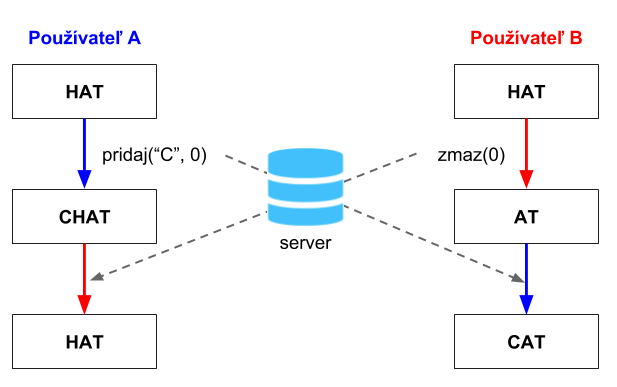
\includegraphics[width=0.6\textwidth]{images/nekomutativne_operacie}}
%popis obrazku
\caption[Nekomutativita textových operácii]{Nekomutativita textových operácii}
%id obrazku, pomocou ktoreho sa budeme na obrazok odvolavat
\label{obr:nekomutativita}
\end{figure}

\begin{figure}[h]
\centerline{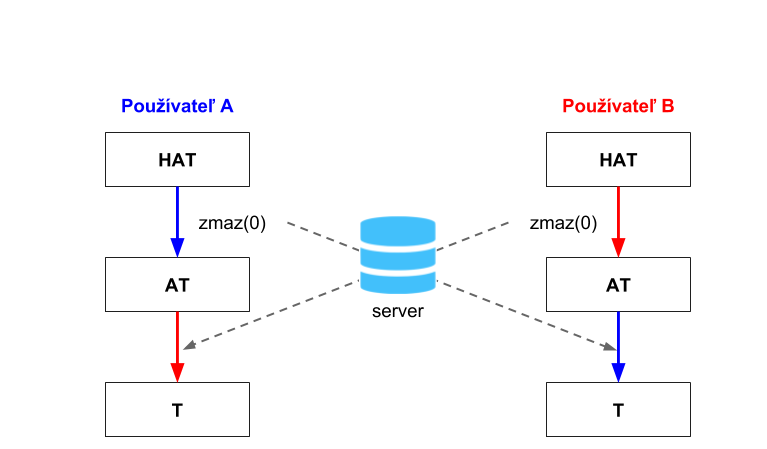
\includegraphics[width=0.6\textwidth]{images/neidempotentne_operacie}}
%popis obrazku
\caption[Neidempotentnosť textových operácii]{Neidempotentnosť textových operácii}
%id obrazku, pomocou ktoreho sa budeme na obrazok odvolavat
\label{obr:neidempotentnost}
\end{figure}

Výzvou v spolupráci v reálnom čase je teda presne zistiť, ako možno aplikovať úpravy
od vzdialených používateľov, ktoré boli pôvodne vytvorené vo verziách dokumentu,
nikdy lokálne neexistovali a môžu byť v rozpore s vlastnými miestnymi úpravami používateľa.

Najsofistikovanejšie riešenia vyriešia tento problém spôsobom, ktorý nevyžaduje server,
nepoužíva uzamknutie (všetci používatelia môžu voľne upravovať všetky časti dokumentu súčasne) 
a podporuje ľubovoľný počet používateľov (obmedzený iba zdrojmi počítačov). 
\textit{UNA} a \textit{SubEthaEdit} sú príklady dvoch programov, ktoré využívajú tento prístup.
Tieto programy sú však dostupné iba pre operačných systémoch macOS a využívajú technológie,
ako napríklad \cite{bonjour},ktoré sú špecifické pre tento operačný systém.

Zatiaľ čo tieto sofistikované prístupy umožňujú najlepšiu používateľskú skúsenosť,
v klientskom serveri môže byť vytvorený aj základný editor pre spoluprácu. Pri klient-server 
scenári je pri otvorení dokumentu priradená jednej z inštancií editora úloha servera.
Tento server zaisťuje, že ostatné editory sú synchronizované. Server obdrží upozornenia
na zmeny vykonané v dokumente inými používateľmi. 
Určuje, ako majú tieto zmeny ovplyvňovať svoju lokálnu kópiu, a vysiela jej zmeny ostatným klientom.
V niektorých modeloch sa zmeny na klientovi neodzrkadľujú dovtedy,
kým sa zo servera nevráti oficiálna odpoveď, a to aj vtedy, ak boli tieto zmeny vykonané lokálne.
Príkladom takéhoto editora je napríklad \textit{Gobby}.

My sme sa v práci rozhodli použiť klient-server model, pričom za synchronizáciu klientov
je zodpovedný výhradne server. Podobný prístup používa napr. spoločnost Google v produkte 
Google dokumenty.

\section{Algoritmy riešiace konkurentné modifikácie}
Na riešenie synchronizácie klientov existujú dva dobre preskúmané typy algoritmov.
\begin{enumerate}
  \item OT - Prevádzková transformácia (Operational transformation)
  \item CRDT - Bezkonfliktné replikovateľné dátové typy (Conflict-free replicated data type)
\end{enumerate}

V práci použijeme CRDT, pretože OT je predchodca CRDT a v praxi často nefunguje tak dobre,
ako to autori zamýšľali. Taktiež použitie OT je komplikované a neškálovateľné \cite{ot_nonscalable}.
